\documentclass[twoside]{protokoll}
\usepackage{graphicx}
\usepackage{tabularx} % for better table formatting
\usepackage{booktabs} % for better table formatting
\usepackage{float} 
\praktikum{I}
\usepackage{subfig}
\usepackage{amsmath}

\versuchsgebiet{(Akustik)}


\teilnehmer{Maximilian Carlos Menke, 434170}
\teilnehmer{Andrea Roth, 428396}
\gruppe{A3}

\begin{document}
 

%\begin{figure}[H]
%  \centering
%  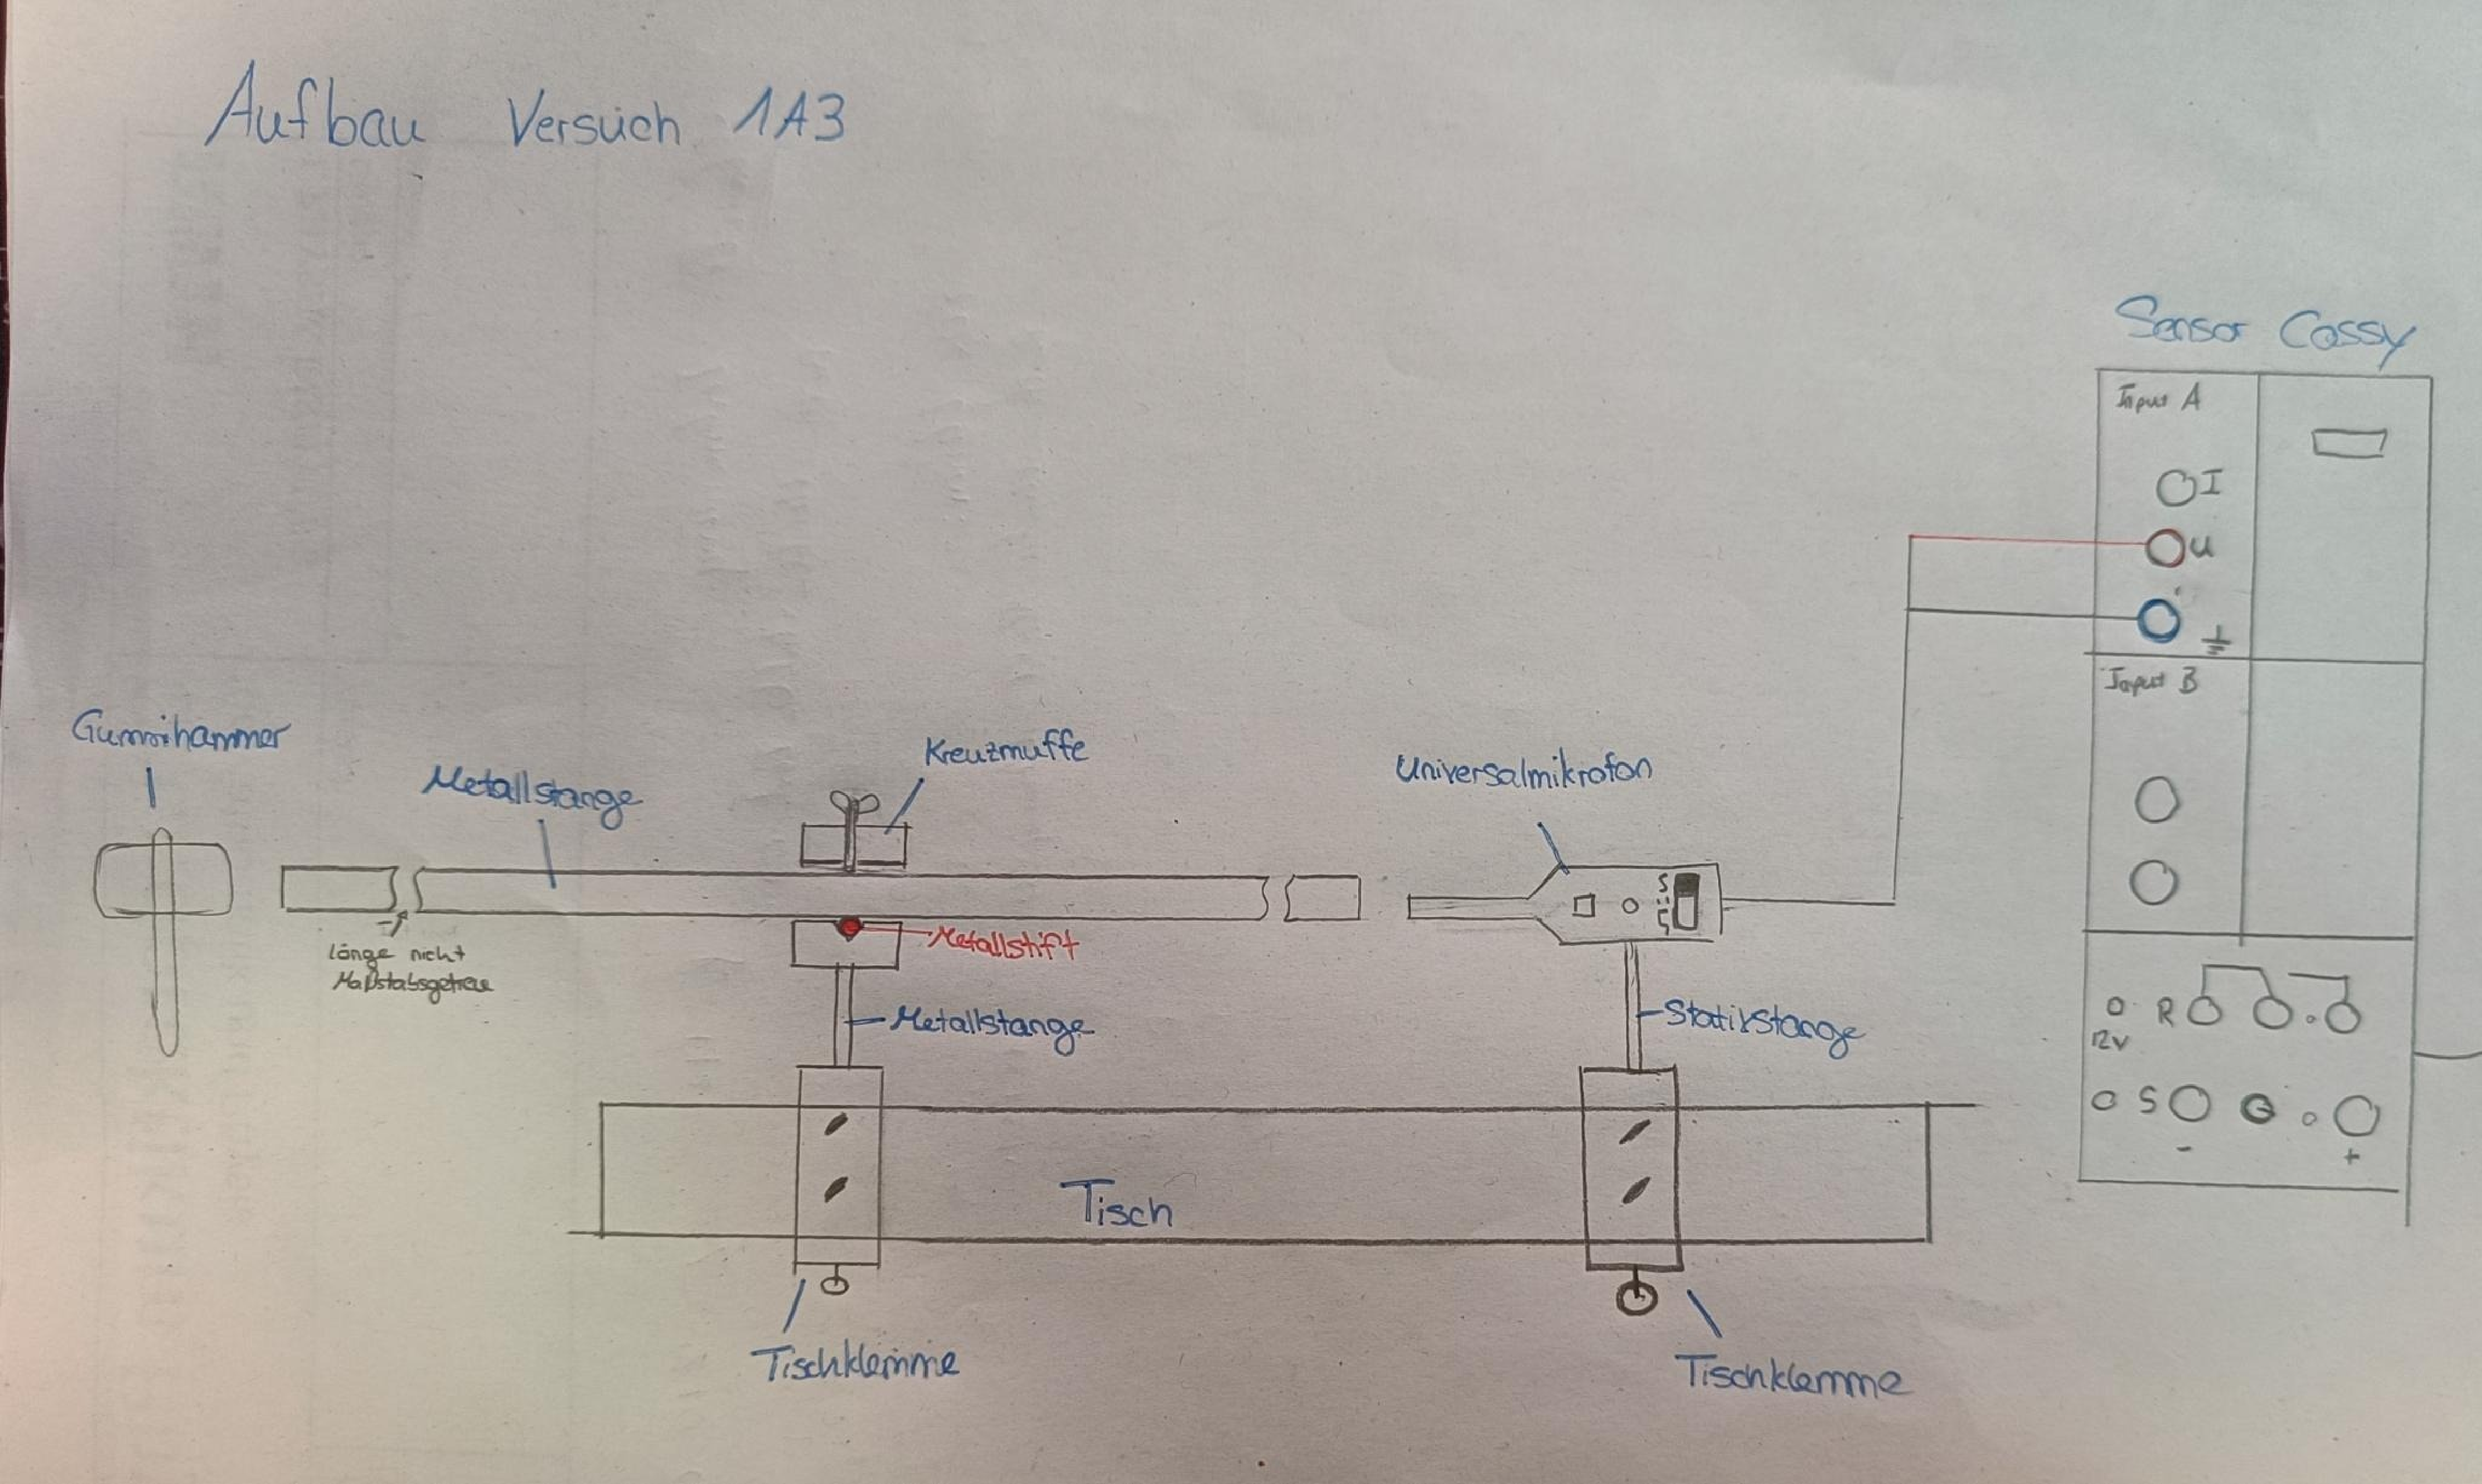
\includegraphics[width=1\textwidth]{Bilder/434170_428396_1A3_SkizzeAufbau.pdf}
%  \caption{Skizze des Versuchsaufbaus}
%  \centering
%\end{figure}

\begin{table}[H]
        \centering
        \begin{tabularx}{0.8\textwidth}{X c c} % adjust width as needed
            \toprule
            \textbf{Metall Stange} & \textbf{Masse} & \textbf{Länge} \\
            \midrule
            Aluminium & 460.9g & 150cm \\
            Messing & 1427.5g & 150cm \\
            Kupfer & 1505.4g & 150cm \\
            Stahl 15 & 1327.4g & 150cm \\
            \bottomrule
        \end{tabularx}
        \caption{Masse und Länge der Stäbe}
        \label{tab:mytable}
    \end{table}


 

\begin{versuchsziele}
\end{versuchsziele}

\section{1E1 Ladekurven eines Kondensators}


\begin{versuchsziele}
Ziel des Versuchs ist die Kapazität eines Kondensators durch lade und entladevorgang
zu bestimmen. 
Dieser wird durch eine Schaltung mit Wiederstand und Schalter bestimmt.
Hierfür werden verschiedene Methoden verwendet. Mit dem Multimeter werden Kapazität
und Wiederstand bestimmt.
Mit dem Osziloskop wird die Kapazität bestimmt. Und mit Sensor CASSY 2 zunächst der 
Wiederstand 
\end{versuchsziele}


\begin{aufgabe}{Grundlagen}
  Knappe Beschreibung der theoretischen Grundlagen, Angabe der
  benötigten Formel(n), ohne Herleitung. Definition der verwendeten
  Formelzeichen.
\end{aufgabe}

% Bitte belassen Sie die Aufgabentexte in Ihrem Protokoll und beginnen
% Sie hier mit der Lösung der ersten Aufgabe:



\begin{aufgabe}{Vorversuch: Charakterisierung der verwendeten Bauteile}
  Charakterisieren Sie die verwendeten Bauteile mit Digitalvoltmeter
  und Messbrücke.
\end{aufgabe}


\begin{aufgabe}{Vorversuch: Bestimmung des Ohmschen Widerstands}
  Beschreiben Sie den Versuchsaufbau unter Verwendung eines
  Schaltbildes. Beschreiben Sie die Versuchsdurchführung unter Angabe
  der relevanten Messwerterfassungseinstellungen. Zeigen Sie
  exemplarisch die Häufigkeitsverteilungen für Spannung $U$ und Strom
  $I$ an einem Messpunkt und beschreiben Sie, wie Sie die
  statistischen Fehler für $U$ und $I$ bestimmen. Tragen Sie die
  Spannung $U$ gegen den Strom $I$ auf und bestimmen Sie aus der
  Steigung den Widerstand $R$ und seine statistische
  Messunsicherheit. Ermitteln Sie den systematischen Fehler mit der
  Verschiebemethode.
\end{aufgabe}


\begin{aufgabe}{Lade- und Entladekurven des Kondensators mit dem Oszilloskop}
  Beschreiben Sie den Versuchsaufbau unter Verwendung eines
  Schaltbildes. Beschreiben Sie die Versuchsdurchführung unter Angabe
  der relevanten Messwerterfassungseinstellungen. Zeigen Sie für den
  Lade- und den Entladevorgang jeweils ein Bild der gemessenen
  Spannungsverläufe auf dem Oszilloskopschirm. Lesen Sie mithilfe der
  Cursor jeweils die Zeitkonstante ab. Berechnen Sie den gewichteten
  Mittelwert der Zeitkonstanten. Berechnen Sie daraus die Kapazität
  und geben Sie sie mit statistischer und systematischer
  Messunsicherheit an.
  
  Für diesen Teil des Gesamtversuchs benötigen wir folgende Geräte:
  
  \textbf{Benötigte Geräte:}
  \begin{itemize}
  	\item TDS 200 4B Oszilloskop
  	\item Sensor CASSY 2
  	\item Rastersteckplatte DINA A4
  	\item 10 $\mu$F Kondensator
  	\item 1 k$\Omega$ Wiederstand
  	\item Brückenstecker
  	\item 3 Kabel rot / blau
  	\item Taster
  \end{itemize}   

  Wir haben uns entschieden den Gesamten Versuch mit einem 10$\mu$F Kondensator und einem 
  1 k$\Omega$ Wiederstand durch zu führen. Hierfür haben wir uns entschieden, da dies dazu
  führt, dass wir eine größere Zeitkonstante haben. Dies ist erwünschenswert, da der 
  Lade/Entlad  Vorgang so langsamer verläuft. Somit haben wir eine Höhere Auflösung 
  der Messungen dies Verringert den Fehler. Allerdings führt dies auch dazu, dass nur wenig
  Strom durch den Wiederstand fließt. Ein großer Wiederstand erhöht also auch den Fehler auf 
  den Strom den wir später mit dem Sensor CASSY messen, da dieses nicht beliebig kleine 
  Ströme messen kann. Hier ist ein größeres $\tao$
  
  der Obigen Skizze können Sie das Schaltbild zu dem Versuch sehen. 
  Auf dem Steckbrett werden hierfür Kondensator und Wiederstand in Reihe gesteckt.
  Parallel zu dem Kondensator wird ein Schalter eingebaut, der bei bedarf den Stromkreis
  schließen kann. Ebenfalls paralell wird eine Spannungsquelle angeschlossen. 
  Hier wird das Sensor CASSY als Spannungsquelle Verwendet 
\end{aufgabe}


\begin{aufgabe}{Lade- und Entladekurven des Kondensators mit Cassy}
  Zeigen Sie für den Lade- und den Entladevorgang jeweils ein Bild des
  Spannungsverlaufs am Kondensator und des Lade- bzw.~Entladestroms.
  Korrigieren Sie erforderlichenfalls den Spannungs- und/oder
  Strom-Offset. Transformieren Sie die Rohdaten geeignet in
  logarithmische Größen und bestimmen Sie mittels linearer Regression
  die Zeitkonstante. Beschreiben Sie, wie Sie die Messunsicherheiten
  behandeln. Berechnen Sie das gewichtete Mittel und geben Sie Ihr
  Endergebnis für die Kapazität mit statistischer und systematischer
  Messunsicherheit an.
\end{aufgabe}


\begin{aufgabe}{Zusammenfassung und Diskussion}
  Fassen Sie Ihre Ergebnisse zu den Kapazitäten zusammen und
  vergleichen Sie sie untereinander, mit den Messungen aus dem
  Vorversuch und mit den Herstellerangaben (Toleranz
  $\SI{5}{\percent}$).  
\end{aufgabe}

 
 
 
\end{document}
